\chapter{Multiple Cameras for SLAM}
\label{chapter:MultiCamSLAM}

\section{Motivation}

There has been significant research in the area of visual SLAM for stereo cameras (cite, cite, cite).  Stereo SLAM has been shown to work very well, however there are a few intrinsic drawbacks of using projective cameras, mainly, the limited field of view.  A larger field of view allows features to be tracked for much longer, which in turn provides much more accurate point triangulation.  In addition to better triangulation, a larger field allows greater overlap of frames, particularly with rotational motion.  This allows for more robust pose estimation and easier localization against an existing map. %occlusions?
%TODO:: citation

Using an omni-directional lense allows a 360$^{\circ}$ view from a single frame.  Such a camera is ideal for doing visual SLAM.  However doing SLAM with a single camera has its own pitfalls.  Firstly the maps and trajectory for mono SLAM will be determined in some non metric scale.  When using stereo, one can determine exact 3D locations of landmarks based on the disparity and a known baseline.  However with a single camera a feature point could lie anywhere on a ray from the focal center to infinity.  Using the 5 point algorithm (cite, reference), 3D positions of points of 2D-2D correspondences between two image frames may be estimated, along with a transformation, however this 3D information is represented in some non metric scale.

\begin{figure}[h!]
  \centering
    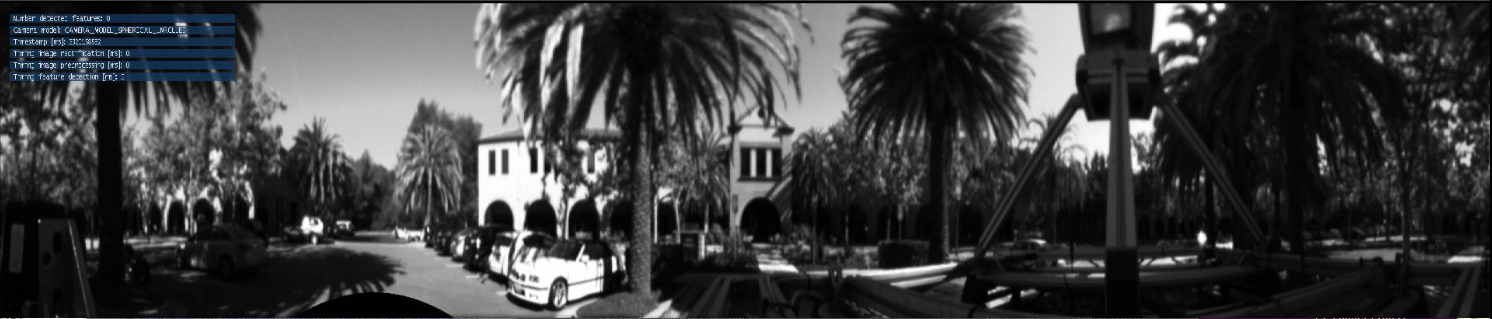
\includegraphics[width=1.0\textwidth]{chapters/images/unwrapped}
    \caption{Omni-lense image unwrapped to panoramic picture}
  \label{fig:unwrapped}
\end{figure}

The second main problem with mono SLAM is scale drift.  Once a pose between two initial images has been calculated, further images need to be registered to this same scale.  The p3p algorithm (cite, reference) calculates a pose for 2D-3D correspondences, propagating the same scale for the new landmarks.  However even a very small error in the scale estimation will cause scale drift over many frames, just as the 3D pose will also drift over long trajectories.

Therefore in order to make a more robust, accurate SLAM system, it would make sense to combine these two types of cameras to exploit their complimentary benefits.  For smaller robots requiring minimal navigation solutions this may not be suitable, however for larger robotic platforms that require highly accurate navigation, for instance self driving cars, robot forklifts or farming robots, this would be an ideal solution.  Two cameras is clearly more expensive than one, however such a localization solution is still much cheaper than high end laser localization systems.

%Talk about the pros and cons of both cameras.  In short 
%\begin{center}
 %\begin{tabular}{ | l | p{5.5cm} | p{5.5cm} | }
  %\hline
  %\bf Camera & \bf Pros & \bf Cons \\ \hline
  %omni 
  %& sees 360 degrees, \newline 
  %tracks points for longer \newline
  %orientation invariant place recognition
  %& non metric scale \newline 
  %scale drift \newline less robust pose estimation\\ \hline
  
  %stereo 
  %& 3D data \newline metric scale \newline no scale drift
  %& small fov \newline
  %more susceptible to occlusions \newline 
  %tracks features not as long \newline 
  %harder to get an even distribution of features \\ \hline
 %\end{tabular}
%\end{center}
%Therefore combine them to get the ultimate visual slam setup!

\section{Approach}

There are many ways in which stereo and omni directional cameras could be fused together.  This section lists some approaches and discusses the selected strategy.

\subsection{Augment Mono-SLAM with stereo}

A fairly straight forward approach would be to use a SLAM algorithm designed for mono slam and address the scale issue with stereo.  Metric 3D points can be determined from stereo and matched to 2D points from the omni directional image.  All points and poses may then be initialized to metric scale.  At any point in time the the scale from the mono system can be compared with metric scale and corrected, given there is some overlap field of view between the two cameras and some feature matches.

\subsection{Augment Stereo-SLAM with an Omni camera}

\subsubsection{Improve Visual Odometry}

A potential improvement to stereo tracking would be to initialize landmarks with stereo and continue to track them as they go out of the stereo camera's field of view with the omni camera.  The p3p algorithm could be used with 3D-2D correspondences to calculate a pose.  Alternatively these points could be considered in the RANSAC pose estimation step by calculating reprojection error for a given pose and then either counting them as inliers or outliers.

\subsubsection{Omni-camera for loop closure (fuck yeah!)}

The idea here is to use the omni camera to find global loop closures where the stereo camera normally wouldn't.  The omni directional can match frames regardless of rotation about the upward facing axis, due to the 360$^{\circ}$ view.  (fig \ref{fig:omni_loop_close}) This means that for robots driving on a ground plane, it could recognize and even match frames regardless of the robots orientation.

\begin{figure}[h!]
  \centering
    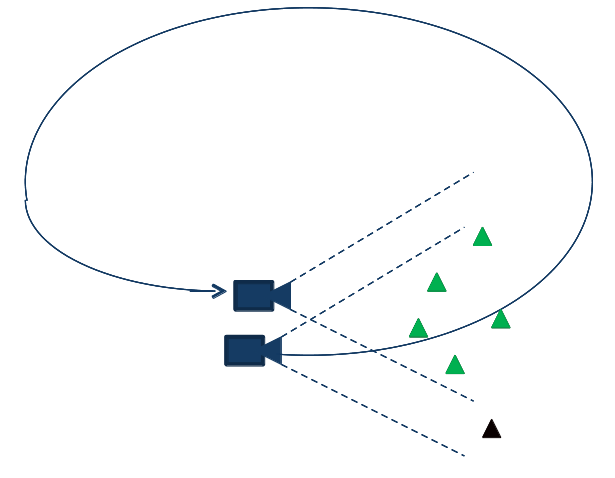
\includegraphics[width=0.49\textwidth]{chapters/images/stereo_loop}
    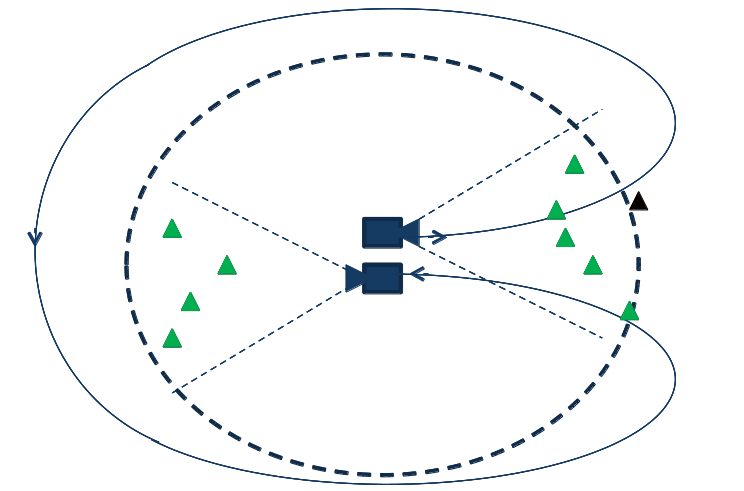
\includegraphics[width=0.49\textwidth]{chapters/images/omni_loop} 
    \caption{Loop closure using a perspective (e.g. stereo) camera and omni-camera.  The omni camera can find loop closures regardless of the cameras pose}
  \label{fig:omni_loop_close}
\end{figure}

\subsection{Tight integration of all cameras}

Another idea is to combine all camera images at the lowest level to enable a tight sensor integration.  A naive implementation of this would be to use a mono SLAM system and treat the images from extras cameras as extra frames.  This could be improved upon by considering the fixed geometry between cameras.

\subsection{Selected Approaches}
\label{subsec:selected_approach}

When developing an online SLAM system, a very important factor to consider is visual odometry drift.  Even with high accuarcy tracking, there will always be some small error which will propagate and over time and cause the trajectory and map to deteriorate. It is likely that tracking accuracy and robustness can be improved by combining stereo and omni cameras in the visual odometry stage, however drift will still occur.

Therefore it is conceivable that the most significant improvement may be made by improving the instances and quality of loop closures to correct for drift.  As a result the Omni camera for loop closure has been selected as the approach for this work.  However this approach is not so trivial, as the non metric scale issues still exists.  This problem will be addressed in this work.

In addition to this approach, a naive combination of all cameras in a mono SLAM framework is very straight forward, given a working SLAM system.  Therefore this method will also be evaluated using an existing mono SLAM framework.
